% begin module net-change-physics
\begin{frame}
\begin{itemize}
\item  If an object moves along a straight line with position function $s(t)$, then its velocity is $v(t) = s'(t)$.
\item  In this case, the Net Change Theorem says
\[
\int_{t_1}^{t_2} v(t) \diff t = s(t_2) - s(t_1).
\]
\item<2->  This is the displacement, or net change of position.
\item<3->  If we want to calculate the distance the object travels, we have to consider separately the intervals where $v(t) \geq 0$ (object moves to the right) and $v(t) \leq 0$ (object moves to the left).
\end{itemize}
\vspace{-.5cm}
\begin{columns}
\column{.55\textwidth}
\uncover<4->{%
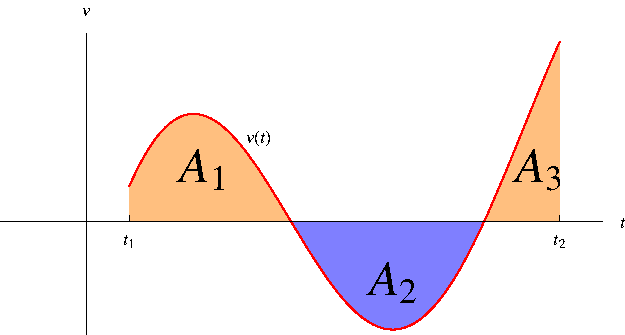
\includegraphics[width=6cm]{integration/pictures/05-04-distance.pdf}
}%
\column{.45\textwidth}
\uncover<4->{%
\begin{eqnarray*}
\textrm{displacement} & = & \int_{t_1}^{t_2} v(t) \diff t\\
& = & A_1 - A_2 + A_3\\
\textrm{distance} & = & \int_{t_1}^{t_2} |v(t)| \diff t\\
& = & A_1 + A_2 + A_3\\
\end{eqnarray*}
}%
\end{columns}
\end{frame}
% end module net-change-physics
